TODO: rewrite
\begin{itemize}
	\item mention TS-ADC paper from the 90s (technique is already known since then, a lot of development )
	\item briefly explain the evolution over the past 20/30 years
	\item transition to usage of TS in physics
\end{itemize}

Observing non-repetitive and statistically rare signals that occur on short timescales requires fast real-time measurements that exceed the speed, precision and record length of conventional digitizers. Photonic time stretch is a data acquisition method that overcomes the speed limitations of electronic digitizers and enables continuous ultrafast single-shot spectroscopy, imaging, reflectometry, terahertz and other measurements at refresh rates reaching billions of frames per second with non-stop recording spanning trillions of consecutive frames. The technology has opened a new frontier in measurement science unveiling transient phenomena in nonlinear dynamics such as optical rogue waves and soliton molecules, and in relativistic electron bunching. It has also created a new class of instruments that have been integrated with artificial intelligence for sensing and biomedical diagnostics. We review the fundamental principles and applications of this emerging field for continuous phase and amplitude characterization at extremely high repetition rates via time-stretch spectral interferometry.

A new generation of instruments based on photonic time stretch is opening the path to measuring and understanding the behaviour of non-stationary and rare phenomena in ultrafast systems, and harvesting their potential for practical applications such as metrology, machine vision and biomedicine. While these instruments rely on optics for the transformation of a signal's timescale, they are able to operate with either electrical, optical, or terahertz inputs. \cite{szwaj}




\section{Time-Stretching Techniques in Physics}
\begin{itemize}
	\item Relativistic electron beam diagnostics
	\item Characterization of noise and fluctuations in nonlinear optics
	\item Laser dynamics
\end{itemize}


\section{Motivation}

From the student job proposal:

Terahertz science and laser applications need to analyse the characteristics of ultrafast events. Commercially available real-time equipment is limited in bandwidth (240 GS/s, LeCroy LabMaster 10-100Zi) and cannot be used to characterize these events in the pico-and femtosecond regime. In this thesis you will evaluate a real-time measurement technique based on the photonic time-stretch analog-to-digital converter (TS-ADC) for the measurement of ultrafast signals with a sampling-rate which exceeds TS/s. The principle is to use a photonic front-end that effectively “slows down” the analog signal in time before it is digitized by fast ADCs.


\begin{figure}[tbh]
	\centering
	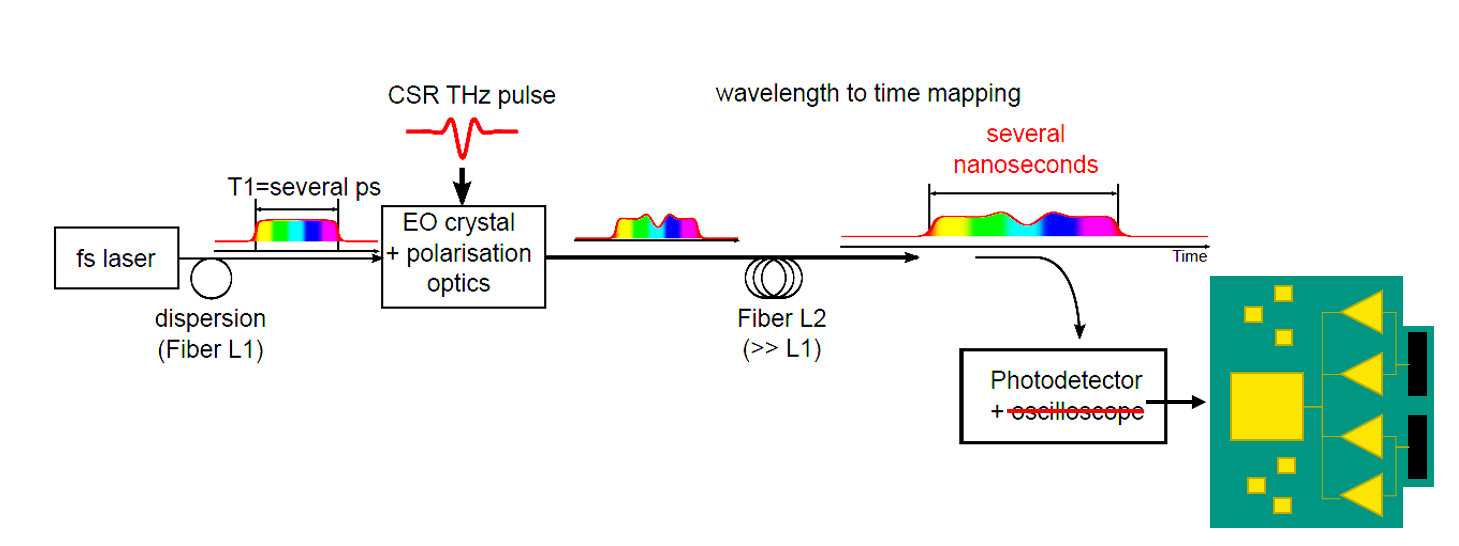
\includegraphics[width=\textwidth]{chap/02-theory/img/motivation}
	\caption{Use case of the system}
	\label{fig:motivation}
\end{figure}
%todo to tikz

\subsection{THz Science and Coherent Synchrotron Radiation}
\textbf{TODO:} Explain physical expressions

\Gls{sr} is produced in synchrotron radiation facilities (like electron storage rings) by accelerating relativistic electrons.
Emission of \gls{sr} occurs, when electron beams are bent or deflected with dipole magnets or using an undulator\footnote{Undulators are used to make the electrons oscillate by generating a periodic magnetic field}. 

\autoref{fig:storageRing} shows the general scheme of an electron storage ring.
Electrons, or rather electron bunches, are generated with an electron gun and are accelerated to almost the speed of light by a \gls{linac}.
After being broad up to their nominal energy in a booster, the bunches are then injected into the storage ring.
In the ring, the path of the electron bunches is altered by bending magnets, guiding them on a circular trajectory.
Due to emission of \gls{sr} at each bend, the electrons lose energy, which has to be compensated for.
This is done by accelerating them with an electric field inside a \gls{rf} cavity.
Not shown in the drawing are the beamlines, which lead the \gls{sr} radiation, or rather chosen wavelength ranges, through an optical system to the respective user experiments. \cite{roussel2014} \cite{rota2018}

\begin{figure}[tbh]
	\centering
	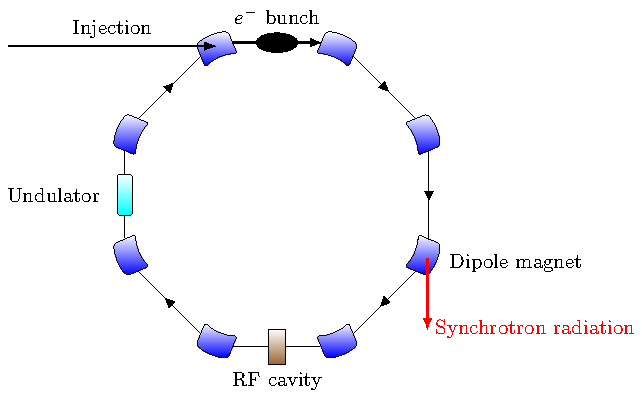
\includegraphics[width=0.7\textwidth]{chap/02-theory/img/synchrotron}
	\caption{Basic scheme of an electron storage ring (redrawn from \cite{roussel2014})}
	\label{fig:storageRing}
\end{figure}
%todo where's the booster?
\paragraph{Karlsruhe Research Accelerator}
\textbf{TODO:} Brief overview over \gls{kara}
\begin{itemize}[noitemsep]
	\item Located at the Karlsruhe Institute of Technology (KIT)
	\item Up to 184 electron bunches can be filled into the storage ring with a distance of \SI{2}{\nano\second} (\SI{500}{\mega\hertz}) between two adjacent bunches
	\item Operated by the Institute of Beam Physics and Technology (IBPT)
	\item Microtron, Booster Synchrotron, and Storage Ring
\end{itemize}

\begin{table}[tbh]
	\caption{KARA parameters \cite{rota2018}}
	\label{tab:kara}
	\centering
	\begin{tabularx}{0.7\textwidth}{Xl}
		\toprule
		\textbf{Parameter} & \textbf{Value} \\
		\midrule
		Beam energy    							&  \SI{2.5}{\giga \electronvolt} \\
		Circumference 	 						& \SI{110}{\meter}	  \\
		Revolution Frequency (one electron)   	& \SI{2.7}{\mega \hertz} 	\\
		Minimum bunch spacing:					& 	\\
		\quad multi-bunch 						& \SI{2}{\nano \second} \\
		\quad single-bunch 						& \SI{368}{\nano \second}	\\
		Bunch length							& \\
		\quad normal operation					& \SI{45}{\pico \second} \\
		\quad short bunch						& \SI{2}{\pico \second} \\
		\bottomrule		
	\end{tabularx}
\end{table}

The range of \gls{sr} reaches from hard X-rays down to the infrared region of the electromagnetic spectrum (see \autoref{fig:spectrum}). In contrast to other sources, it has properties like:
%todo which sources, convert list to text?
\begin{itemize}[noitemsep]
	\item high intensity 
	\item high collimation
	\item polarisation
	\item well-defined timing of pulses
\end{itemize}

Due to this properties, synchrotrons are used for microscopy, spectroscopy, and time-resolved experiments in such fields like condensed matter physics, biology, material science and many more.
%todo why are these imporant for the applications listed here. maybe pick one and explain it in more detail and/or an equation
\begin{figure}[tbh]
	\centering
	\includegraphics[width = \textwidth, height = 0.5\textwidth]{chap/02-theory/img/spectrum.tikz}
	\caption{Electromagnetic spectrum} %todo of what?
	\label{fig:spectrum}
\end{figure}
%todo 7 column not working for some reason, 
%todo replace with measured I(\lambda)/I_0 plot?

\subsubsection*{Micro-Bunching Instabilities}
Increasing demands in current and future accelerators call for higher brilliance of the emitted radiation.
%todo define brilliance, flux, emittance
This is achieved by increased photon flux and reduction of the transverse emittance.
For longitudinal coherence, the electron bunches are shortened, which results in emission of \gls{csr} at frequencies up to the THz range.
%todo how does coherence relate to the terms mentioned earlier?

However, this introduces complex dynamics, as the electrons interact with their own radiation.
This manifests into the so called micro-bunching instability.
The formation of micro-structures (in the sub-millimeter to centimeter range) in the longitudinal density profile of the electron bunches.
Being on the one side a limitation to the stable operation of the overall system at high current density/short bunch length mode.
On the other side, these instabilities can be potential sources of brilliant THz radiation. %todo why
A thorough understanding of these dynamics is necessary to control the emission in this spectral domain which enables usage in experiments. \cite{rota2018,brosi}

\begin{figure}[tbh]
	\centering
	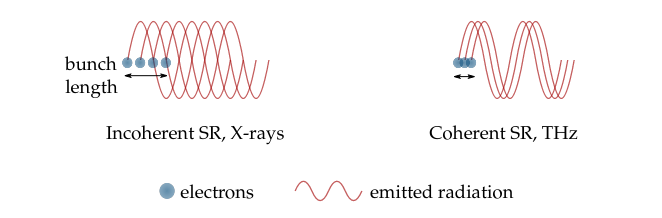
\includegraphics[width = \textwidth]{chap/02-theory/img/csr2.png}
	\caption{Incoherent \gls{sr} and coherent \gls{sr} due to shorter electron bunch length \cite{rota2018}}
	\label{fig:csr}
\end{figure}
%todo to tikz

\begin{figure}[tbh]
	\centering
	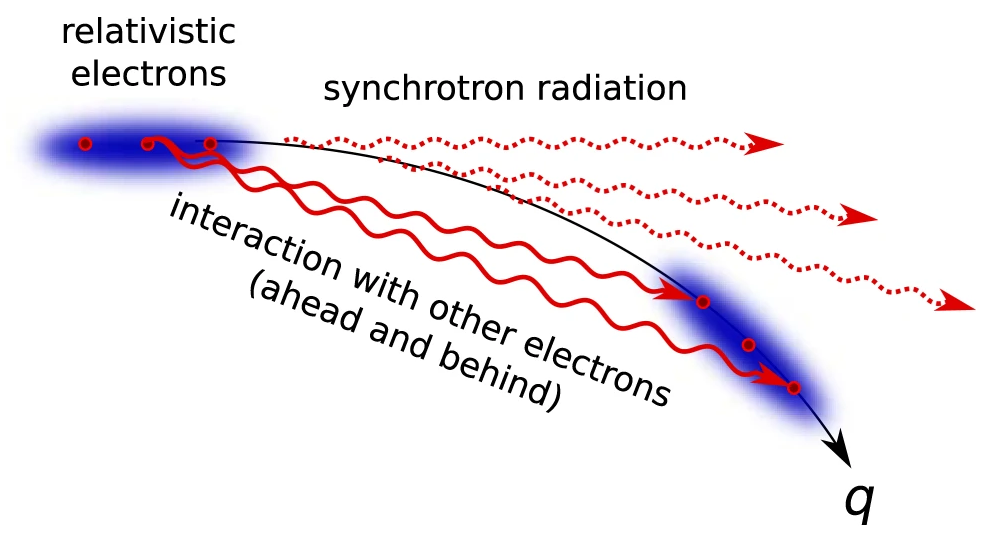
\includegraphics[width = 0.5\textwidth]{chap/02-theory/img/microbunching}
	\caption{Electrons interact with their own radiation \cite{Bielawski2019}}
	\label{fig:microBunch}
\end{figure}


\subsection{Longitudinal Bunch Profile Diagnostics}

\subsubsection*{Scanning-Type Electro-Optic Sampling}
The 
%todo what is that, one sentence
A short laser pulse (duration typically hundreds of femtoseconds) co-propagates with a THz pulse from \gls{csr} (range of picoseconds) in an \gls{eo} crystal. Due to the Pockels effect\footnote{"The Pockels effect denotes the occurrence of
	and change in existing birefringence in an electric field linearly, which is proportional to the electric
	field strength. \cite{pockels}} the THz pulse causes a time dependent birefringence in the crystal.
%todo avoid direct quote
This modulates the polarization of the laser pulse.
To sample the pulse, the delay between the laser and the THz pulse is varied.
To detect the changing polarization, the polarization of the laser pulse is transformed into an intensity modulation.
A general scheme of the system is shown in \autoref{fig:scan_eo}.
For this technique a stable emission of the THz pulses is crucial, as they are not measured in one acquisition. \cite{roussel2014}
\begin{figure}[tbh]
	\centering
	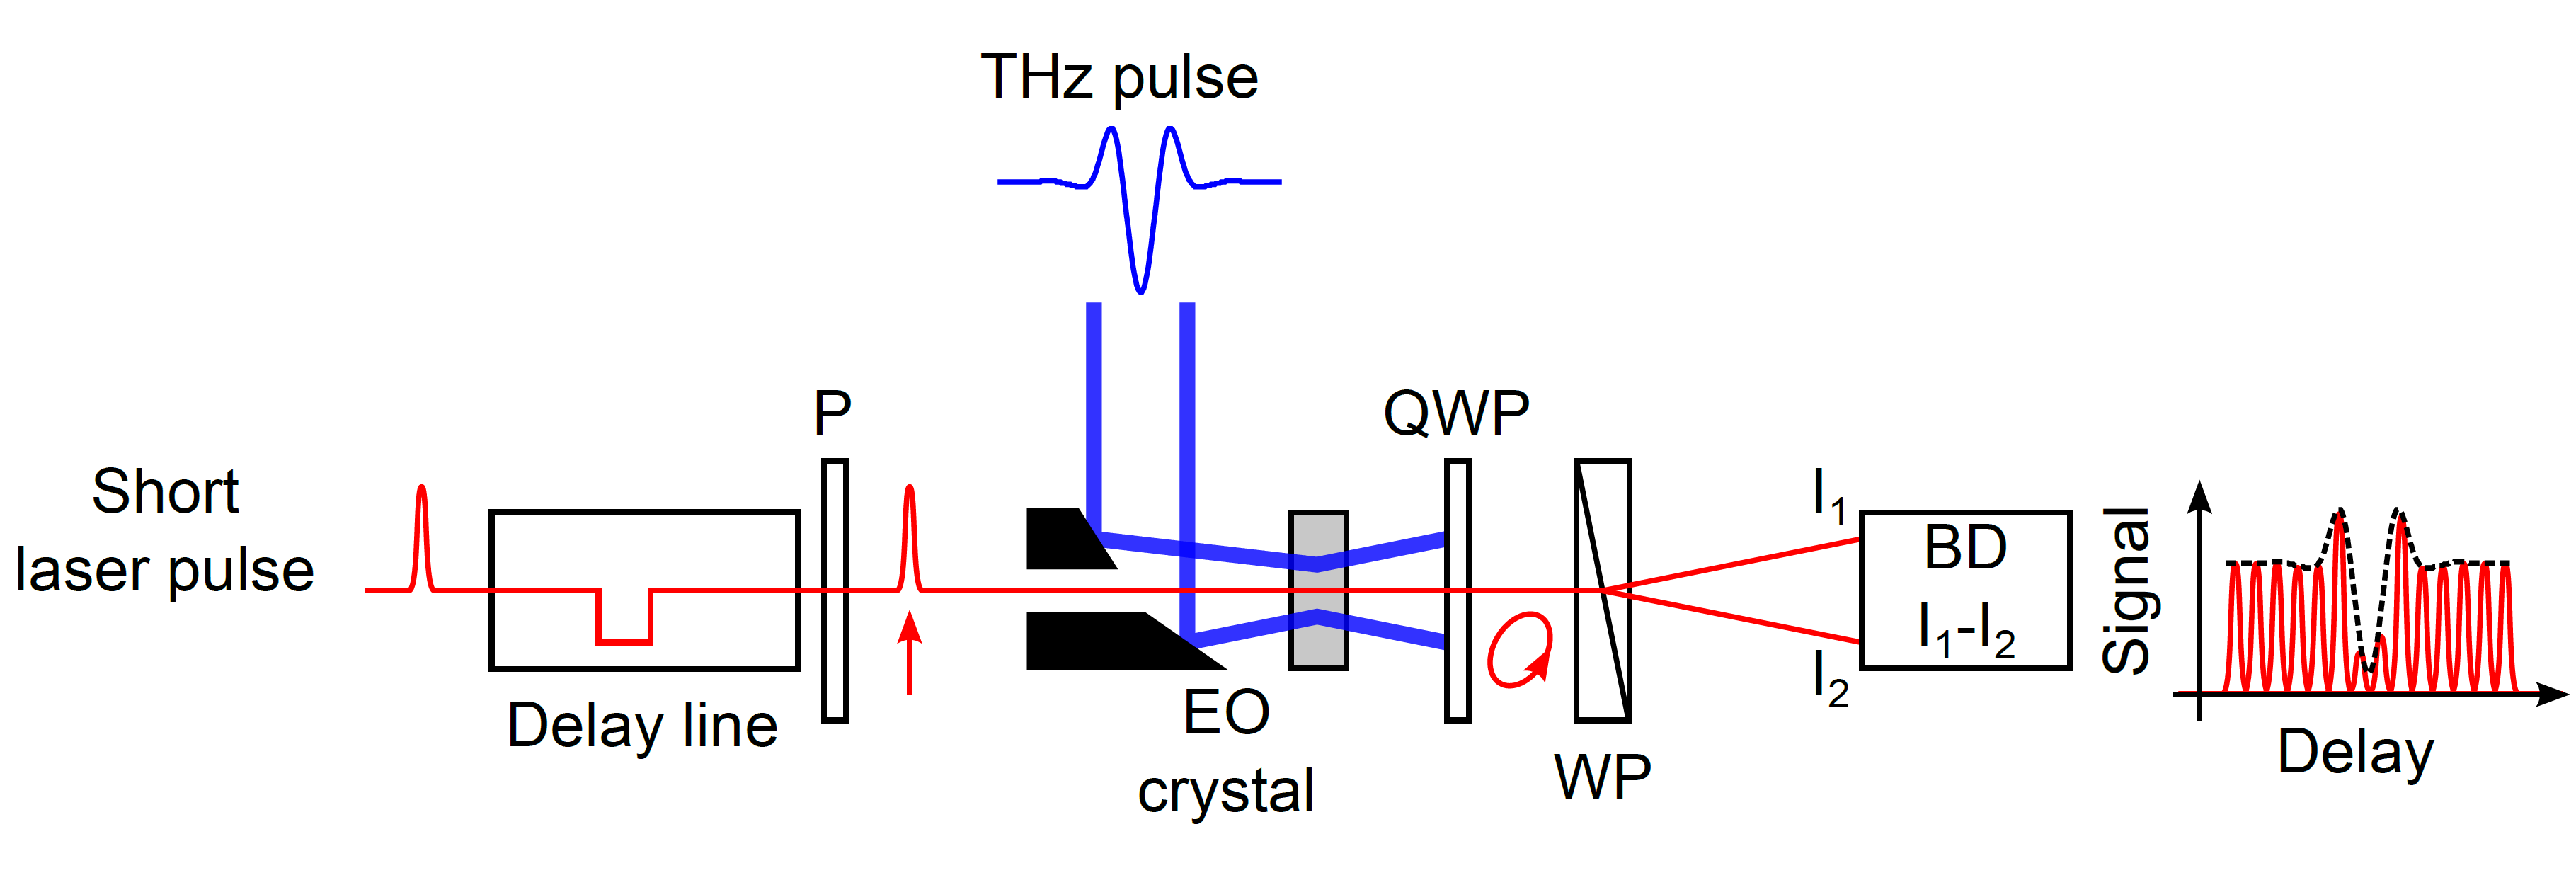
\includegraphics[width = 0.8\textwidth]{chap/02-theory/img/scanning_eo}
	\caption{Scheme of Scanning-Type Electro-Optical Sampling System \cite{roussel2014}}
	\label{fig:scan_eo}
\end{figure}

\subsubsection*{Spectrally Resolved Electro-Optic Detection}
In contrast to the EOS, single-acquisition is possible with the spectrally resolved electro-optic detection technique. %todo EOS==EO?
The short laser pulse is first stretched to a duration similar to the Thz pulse in a dispersive material (stretcher).
In this way the pulse is chirped, meaning the instantaneous frequency of the pulse varies over time.
Together with the THz, the laser pulse propagates in a \gls{eo} crystal.
Again, the induced birefringence modulates the laser pulse, not only in time, but also in the optical spectrum.
The polarization state of the pulse is converted into an amplitude/intensity modulation.
To retrieve the THz pulse shape in time, the spectrum of the laser pulse is measured with a spectrometer. %todo what spectrometer (optical or electrical) or state model
A general scheme of the system is shown in \autoref{fig:spectral_eo}. \cite{roussel2014}

\begin{figure}[tbh]
	\centering
	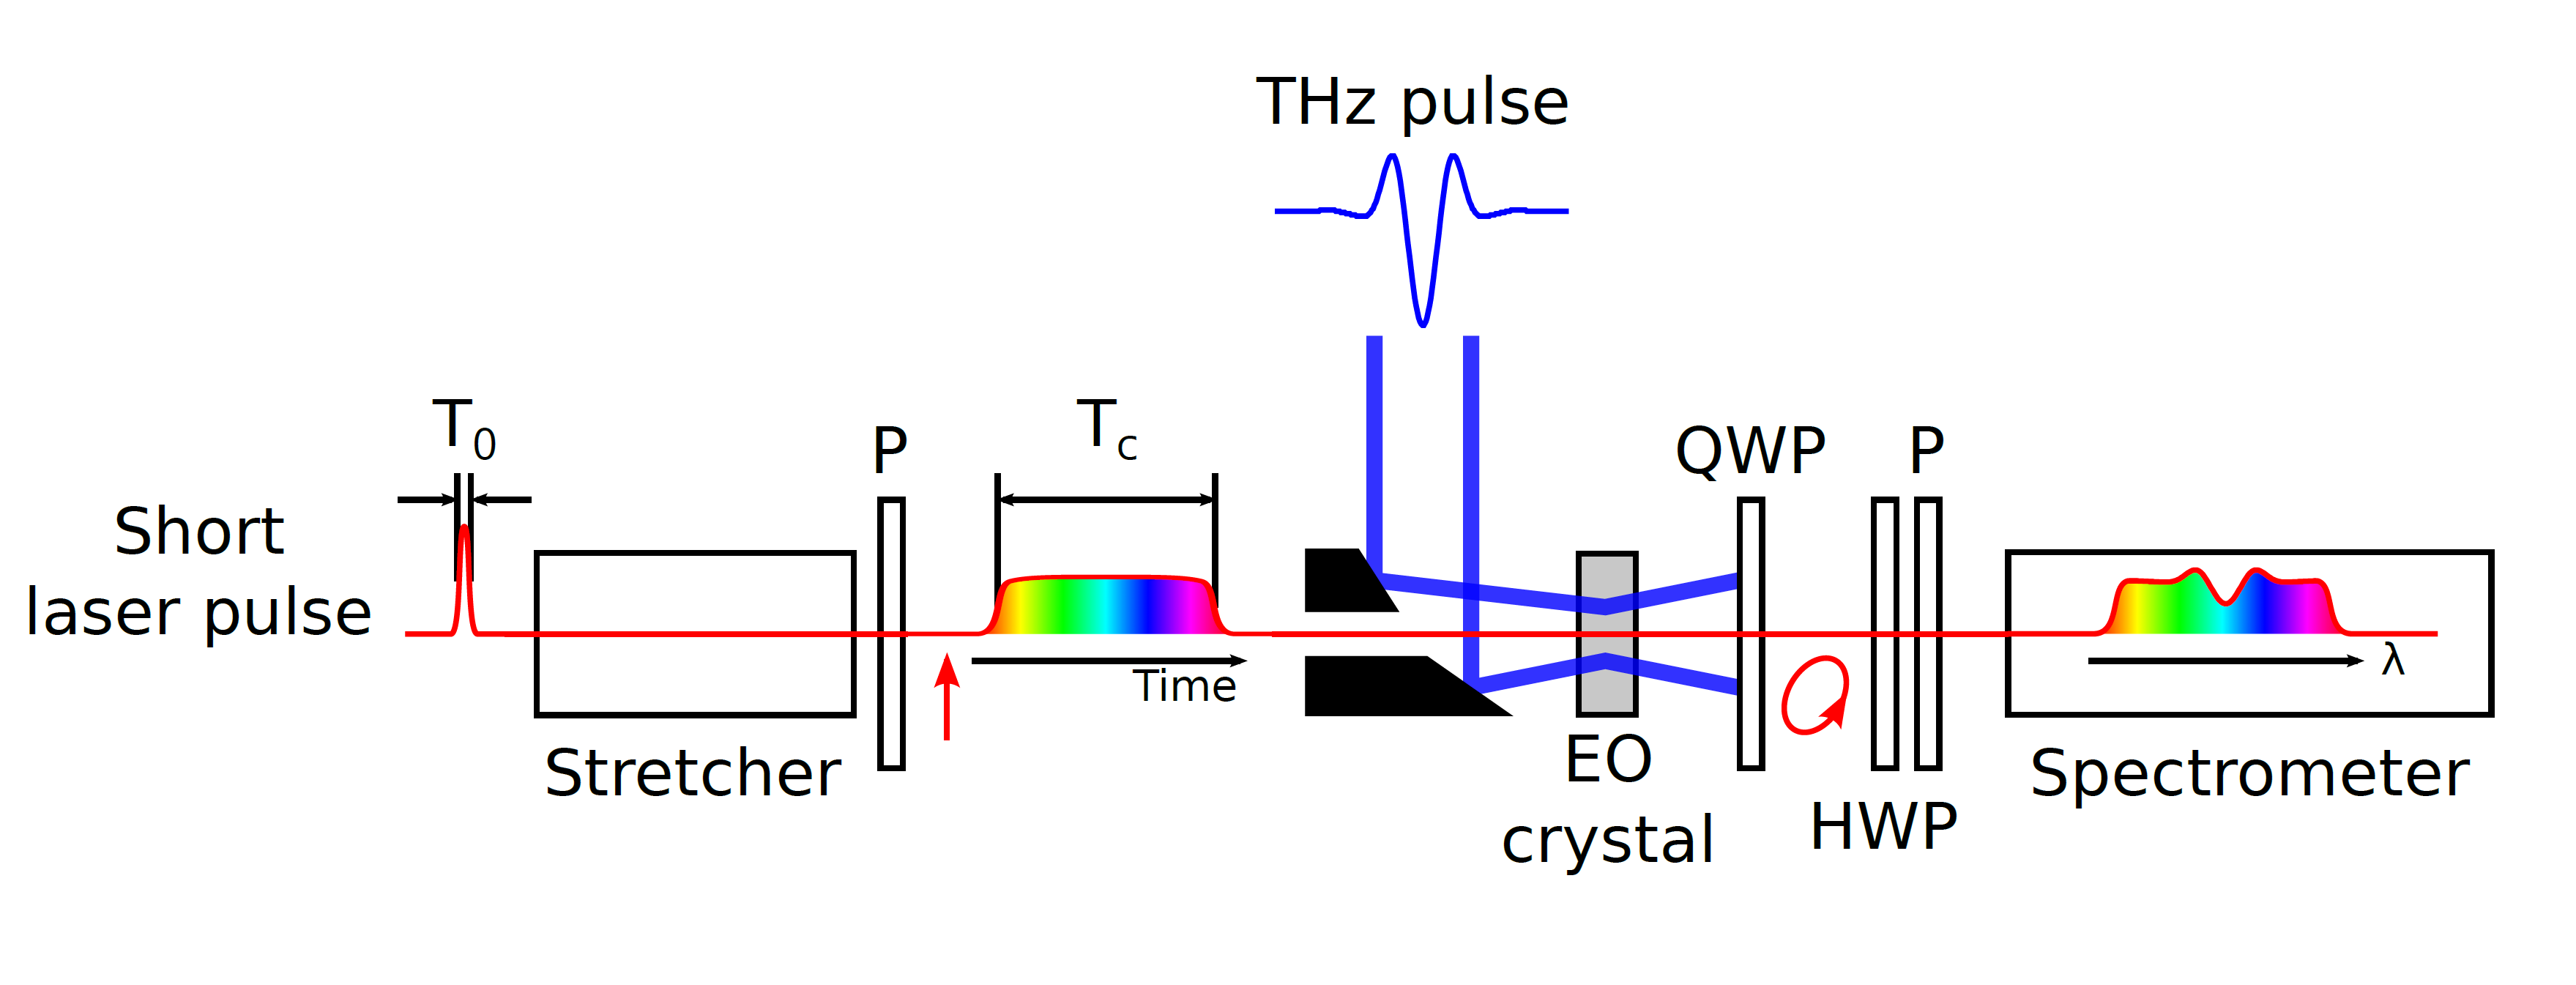
\includegraphics[width = 0.8\textwidth]{chap/02-theory/img/spectral_eo}
	\caption{Scheme of Spactrally Encoded Electro-Optical Detection System \cite{roussel2014}}
	\label{fig:spectral_eo}
\end{figure}

The temporal resolution of this method is limited due to the finite chirp rate
\begin{equation}
	\text{chirp rate} = \frac{\text{laser bandwidth}}{\text{laser pulse duration after stretcher}}.
\end{equation}

The resolution $T_{\text{min}}$ is determined as
\begin{equation}
	T_{\text{min}} = \sqrt{T_0 T_c}
\end{equation}
with the bandwidth-limited pulse duration (before stretcher) $T_0$ and the duration of the chirped laser pulse $T_c$.


\textbf{TODO}: refer also to KALYPSO


\subsection{Potential Usage: ANR-DFG ULTRASYNC project?}
From Serge's email:

For accelerator applications, we have also a project (ANR-DFG ULTRASYNC project) with KARA and SOLEIL.
There is the question of control (i.e., suppression) of the bursts occuring during the microbunching instability. The objective is to obtain a high power and stable coherent emission (at SOLEIL and KARA). For the moment, the only experimental test has been made using a relatively simple feedback:
\begin{itemize}
	\item a bolometer signal as the feedback loop input
	\item a low-cost FPGA (redpitaya) that sends the feedback on the accelerating voltage
\end{itemize}

There are limitations in the maximal bunch charge in the accelerator. So an open question is whether measuring each THz pulse using EO sampling + time-stretch may help to solve this open problem. In clear:

\begin{itemize}
	\item EO sampling + time-stretch as in Eléonore's thesis
	\item association with the new FPGA-based system
	\item finding adequate feedback that is programmed in the FPGA
\end{itemize}
may solve the problem, and allow the control to succeed at the highest currents in SOLEIL. 
Target would be ca. 15 mA for 1 bunch (and feedback control presently works to a little more than ca. 10 mA).

\section{Objective}
Design of a system to be used with photonics time-stretch technique. Fast, continuous sampling of sifnals, integratable in already existing high data-throughput architectures.






%\begin{itemize}
%	\item Microbunching instabilites $\rightarrow$ THz radiation $\rightarrow$ Potential source of brilliant radiation
%	\item Need to be studied to be able to control it
%	\item Time-resolution critical, as instabilities have high bandwidth
%	\item Commercial oscilloscopes don't have enough internal memory
%	\item already developed system KAPTURE/KAPTURE-2 to solve this problem
%	\item however: four/eight points not enough to see the microbunching instabilities
%	\item Concept: combine time-stretch with FPGA $\rightarrow$ THERESA (\textbf{T}era\textbf{He}rtz \textbf{Re}adout \textbf{Sa}mpling)
%	\item EO technique to stretch the signal in time, so requirements on the bandwidth of converters can be relaxed
%	\item more converters, to have more points
%	\item New generation FPGA/SoC for fast readout and high data throughput
%\end{itemize}
%
%Available commercial DAQ system or real-time oscilloscopes for high bandwidth (e.g. above
%40 GHz) are very expensive and, due to limited internal memory and missing fast readout interfaces, are not suitable for long term bunch-to-bunch CSR measurements. To circumvent these limitations a DAQ architecture for fast and continuous sampling of the individual ultra-short THz pulses has been developed.









%
%
%
%
%The past decade has seen the rapid development of CSR studies in many storage
%rings. Despite the large amount of experimental observations, e.g. the recordings
%of coherent THz bursts, lack of direct observation of the electron bunch and its
%microstructures is a main issue to the test and development of the theoretical models.
%Even though in chapter 5 we presented first real-time measurements of CSR
%pulses using a YBCO superconductor-based detector at UVSOR-III, a majority
%of storage rings emits coherent synchrotron radiation at higher frequencies than
%the state-of-the-art oscilloscope bandwidth (currently 65 GHz), e.g. 300 GHz
%at SOLEIL [8],250 GHz at ANKA [2],500 GHz at ELETTRA [5].
%
%Spontaneous formation of small-scale microstructures can have a deleterious effect on electron bunch stability and emission properties, and they are at the same time a tremendous source of coherent radiation in the terahertz domain3,4,5,6,7,8,9,10,11,12,13,14,15,16,17, provided the instability can be mastered. This is the reason why understanding and controlling the interplay between Coherent Synchrotron Radiation (CSR) and the microbunching instability has nowadays become a central open question in the development of synchrotron radiation facilities.
%
%To answer this question, it is essential to develop ultrafast photonic devices for electron bunch shape characterization. The challenges for the photonics community is high, given the need for ultrashort (picosecond or femtosecond) temporal resolution, single-shot operation, at high repetition rates (MHz and more), and given the particularly challenging environment near relativistic electron bunches. Recent advances consequently pushed photonics systems beyond the state of the art. Ultrafast electric-field measurement techniques using femtosecond laser pulses (electro-optic sampling24) have allowed single-shot bunch shape measurements (plural)25, and these techniques have then been extensively investigated and improved this last decade
%
%
%The ULTRASYNC (Exploration et contrôle ULTRArapide de la dynamique des paquets d'électrons dans les sources de lumière SYNChrotron, ANG-DFG) aims to study and control coherent synchrotron radiation (CSR) and microbunching instability. The goal is to obtain a high power and stable coherent emission (KARA and SOLEIL) by feedback control. At SOLEIL, this was already succesfully achieved, still there is a significant limit to the range, where this concept works. One possible way would be to calculate the necessary feedback from a whole THz CSR pulse shape, which would require to record an electro-optical signal (time-stretch). This leads to a possible approach by combining time-stretch and FPGA. 
%
%For the moment, the only experimental test has been made using a relatively simple feedback:
%- a bolometer signal as the feedback loop input
%- a low-cost FPGA (redpitaya) that sends the feedback on the accelerating voltage
%There are limitations in the maximal bunch charge in the accelerator. So an open question is whether measuring each THz pulse using EO sampling + time-stretch may help to solve this open problem. In clear:
%- EO sampling + time-stretch as in Eléonore's thesis
%-> association with the new FPGA-based system
%-> finding adequate feedback that is programmed in the FPGA
%may solve the problem, and allow the control to succeed at the highest currents in SOLEIL. 
%Target would be ~15 mA for 1 bunch (and feedback control presently works to a little more than ~10 mA).
%
%At 1 micron wavelength, the maximum stretch is limited due to fiber glass properties (at this wavelength). The maximum length achieved are 2-4 ns (SOLEIL and KARA). For this reason, a fast ADC is critical, to get a good ENOB/number of sampling points. A relevant figure of merit (that characterizes the effective number of points) is -- we think: FOM=electronic bandwidth x stretch time. There is some bottleneck concerning time-stretch at this wavelength, and one way to solve the issue is to try pushing the bandwidth of ADCs.
%
%At 1550 nm wavelength, it is possible to stretch the signal up to tens of nanoseconds. Therefore, a relatively cheap ADC would already be sufficient and allow an effective number of samples at around 100. Applications still need to be investigated.
%
%As potential applications for the new system would be applications for accelerators in the 1 micron wavelength (best concerning EO sampling SNR and bandwidth).
%
